\section{دسترس‌پذیری}

دسترس‌پذیری یا \lr{Availability}  یعنی زمانی که می‌خواهیم از چیز استفاده کنیم و
آن چیز بایستی ارائه سرویس را انجام دهد.

\begin{equation}
    Availability = \frac{uptime}{Total Service Time}
\end{equation}

\subsection*{مثال}

یک ماشین هر یک ساعت، ۶ دقیقه داون است. مطلوب است محاسبه \lr{Availability} و
\lr{Reliability}:

\begin{equation}
    Uptime = 60-6 = 54
\end{equation}

\begin{equation}
    Availability = \frac{Uptime}{Total Service Time} = \frac{54}{60} = 0.9 or 90\%
\end{equation}

برای محاسبه قابلیت اطمینان می‌توان گفت که وقتی در یک ساعت ۶ دقیقی با قطع کارکرد
خودرو همراه هستیم، پس قابلیت اطمینان زیر یک ساعت یا کمتر از ۵۴ دقیقه است.

\subsection{بازه زمانی یا \lr{Total time}}

در دسترس‌پذیری بررسی \lr{Total time} بسیار مهم است، چرا که سرویس در آن زمان
بایستی بدون مشکل در دسترس باشد و به صورت صحیح تا انتهای بازه مشخص \lr{Total
time} به کار خودش ادامه دهد. برای مثال سیستم آموزشیار بایستی در ابتدای ترم جهت
اخذ واحد درسی دانشجویان، در یک بازه یک ماهه به طور مثال کاملاً در دسترس و قابل
اطمینان باشد. اما با تغییر دامنه از سیستم انتخاب واحد دانشگاه به دامنه بانکی این
گفته صادق نیست، زیرا محصولات و سرویس‌‌های بانکی بایستی ۲۴ ساعته ۷ روز هفته در
دسترس باشند و کاملاً قابلیت اطمینان را به همراه داشته باشند.

\subsection{ارتباط میان \lr{Availability} با \lr{Reliability}}

عموماً وقتی سیستمی \lr{Reliable} است یعنی دارای \lr{Availability} بالایی است اما
وقتی سیستمی \lr{Available} است ممکن است آن سیستم قابل اطمینان باشد و ممکن است
قابل اطمینان نباشد. زمانی کاملاً قابل اطمینان است که تمام آن سیستم با آزمون‌ها و
ارزیابی‌ها پوشش داده شده باشد و فاقد هر گونه \lr{Fault} باشد و از سمتی در هنگام
استقرار نیز تمام نکات \lr{Availability} به عنوان ویژگی کیفی رعایت و پیاده‌سازی
شده باشند. به این صورت هم دسترس‌پذیری بالایی خواهد داشت هم از قابلیت اطمینان
بالایی برخوردار خواهد بود.

\subsection*{نکته}

در قابلیت اطمینان وابستگی به موقعیت می‌تواند عامل مشخص‌کننده‌ای باشد. برای مثال
با استفاده از یک موتور شارژی می‌توان درون شهر فعالیت کرد، اما با همان موتور
شارژی نمی‌توان به جنوب کشور سفر کرد.

\begin{equation}
    Availability = Reliability + Repair
\end{equation}

\subsection{\lr{Mean Down Time (MDT)}}

میانگین زمانی که یک سیستم قابل استفاده نباشد. \lr{MDT} با فاکتور‌های زیر همراه
است:

\begin{itemize}
    \item \lr{System failure}:
    \begin{itemize}
        \item سیستم به طور کلی فاقد هر گونه \lr{Fault} باشد.
        \item منتظر تامین قطعات نباشد
        \item سیستم نیاز به تعمیر داشته باشد.
    \end{itemize}
    \item \lr{Scheduled downtime}:
    \begin{itemize}
        \item نگهداری پیشگیرانه
        \item به روزرسانی سیستم
        \item کالیبراسیون
        \item سایر اقدامات اداری (\lr{Administrative})
    \end{itemize}
\end{itemize}

مقدار \lr{MDT} هر چقدر کمتر باشد دسترس‌پذیری نیز بیشتر خواهد بود.

\subsection{بدست آوردن مدت زمان \lr{Down time}}

برای محاسبه مدت زمان قطع سرویس یک سیستم از فرمول زیر استفاده کنیم:

\begin{equation}
    (Availability - 1) * Total Time = DownTime
\end{equation}

اگر یک سیستم در یک سال $99.99\%$ دسترس‌پذیری داشته باشد چند دقیقه \lr{Down time}
خواهد داشت:

\begin{equation}
    (0.9999 - 1) * 365D = Down Time
\end{equation}

\begin{equation}
    (0.0001) * 8760Hr = 0.876Hr
\end{equation}

\begin{equation}
    0.876Hr \rightarrow 52.56Min
\end{equation}

\begin{equation}
    52.56Min \rightarrow 52 Min \rightarrow 0.56Min
\end{equation}

در نهایت پاسخ ۵۲ دقیقه و ۳۴ ثانیه قطعی سرویس با $99.99\%$ دسترس‌پذیری می‌باشد.'

\subsection{تعریف کیفیت}

در استاندارد \lr{IEEE 1990} کیفیت به دو صورت تعریف می‌شود:

\begin{enumerate}
    \item چقدر یک سیستم، یک مولفه یا یک فرایند در برابر رویارویی با نیازمندی‌های
    پروژه موفق بوده است.
    \item چقدر یک سیستم، یک مولفه یا یک فرایند در برابر با رفع نیاز‌های کاربران
    موفق بوده است.
\end{enumerate}

\subsection{خصوصیات کیفی قابل مشاهده در زمان اجرای نرم‌افزار}

\begin{enumerate}
    \item کارایی
    \item امنیت
    \item قابلیت استفاده
    \item قابلیت دسترسی
\end{enumerate}

\subsection{خصوصیات کیفی غیرقابل مشاهده در زمان اجرای نرم‌افزار}

\begin{enumerate}
    \item قابلیت اصلاح
    \item قابلیت آزمایش
    \item قابلیت استفاده مجدد
    \item قابلیت یکپارچگی
    \item قابلیت حمل
\end{enumerate}

\subsection{سناریو‌های خصوصیات کیفی}

\subsubsection{\lr{Source of Stimulus} یا منبع تحریک}

منبع تحریک شامل بعضی از موجودیت‌ها از قبیل، انسان، سیستم کامپیوتری، نرم‌افزار‌ها
و هر محرک دیگری است که یک تحریک را در سیستم ایجاد می‌کند یا به بیانی دیگر موجب
تولید یک تحریک می‌شود.

\begin{itemize}
    \item در درخواست کارنامه توسط دانشجو، دانشجو منبع تحریک می‌باشد.
    \item در چاپ شهریه منبع تحریک کسی است که درخواست آن را ارسال می‌کند.
\end{itemize}

\subsubsection{\lr{Stimulus} یا محرک}

محرک وضعیتی است که درسیستم ایجاد شده است و لازمه مورد بررسی قرار گرفتن (باید به
آن پاسخ داده شود) می‌باشد.

\subsubsection{\lr{Environment} یا محیط}

محیطی که در آن منبع تحریک یک وضعیتی یا محرکی ایجاد کرده است. برای مثال زمانی که
یک تحریک رخ می‌دهد ممکن است سیستم در حال اجرا باشد، یا هر وضعیت دیگری مانند
\lr{Shotdown} یا \lr{Standby}.

\subsubsection{\lr{Artifacts} یا فرآورده‌ها}

موجودیتی است که روی آن تحریکی انجام شده است. فرآورده ممکن است کل سیستم یا بخشی
از آن باشد.

\subsubsection{\lr{Response} یا پاسخ}

پاسخ فعالیتی است که سیستم بعد از تحریک شدن انجام می‌دهد.

\begin{itemize}
    \item پیام مناسبی را به کاربر نشان بدهد.
    \item سیستم زیر بار محاسباتی شدید است، در زمانی مشخص پیام دهد که «چند دقیقه
    بعد برای ورود تلاش کنید».
\end{itemize}

\subsubsection{\lr{Response Measure} یا معیار پاسخ}

وقتی که پاسخی بعد از تحریک شدن داده می‌شود باید بتوان آن را به روشی مناسب و مشخص
اندازه‌گیری کرد تا نیازمندی‌های مورد نظر بتواند مورد آزمایش قرار بگیرند.

\subsubsection*{نکته}

\begin{itemize}
    \item تمامی منابع تحریک و محرک‌ها قابل بررسی نیستند.
    \item محیط همیشه بار کاری نیست.
\end{itemize}

\begin{figure}[H]
    \centering
    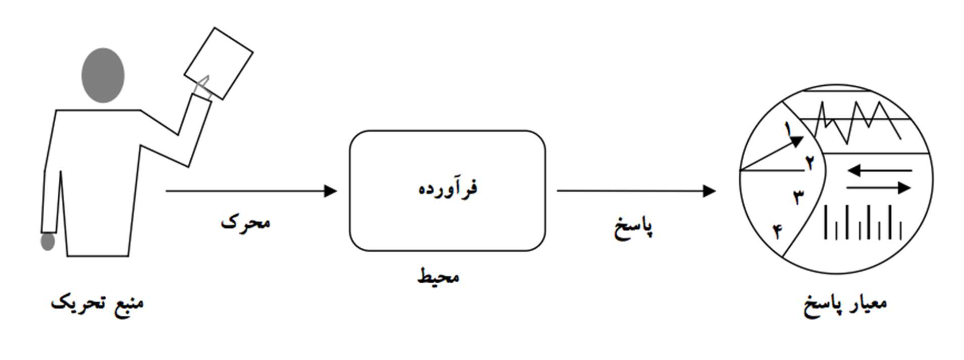
\includegraphics[width=0.8\textwidth]{images/main_section_of_general_scenario.png}
    \caption{بخش‌های اصلی سناریو خصوصیات کیفی}
    \label{fig:generalScenarioMainSections}
\end{figure}

\subsection{\lr{General scenario} یا سناریو عمومی}

سناریو عمومی برای هر ویژگی کیفی \footnote{\lr{Quality attributes}} یک معیار
می‌باشد و فاقد از ویژگی‌های دامنه هر جایی یک سناریو دارد. یا به عبارتی دیگر،
سناریو‌های عمومی مستقل از سیستم هستند و در ارتباط با هر سیستمی می‌توانند باشند.

\subsection{\lr{Concrete scenario} یا سناریو عینی}

سناریو‌های عینی براساس ویژگی‌های دامنه هر پروژه‌ای متفاوت می‌باشند یا به عبارتی
دیگر برای سیستم‌های خاص مشخص می‌شوند.

\subsection*{نکته}

\begin{itemize}
    \item خصوصیات کیفی در سناریو‌های عمومی و عینی دقیقاً مانند هم هستند فقط
    موارد‌ آن‌ها نسبت به دامنه متفاوت مطرح می‌شوند.
    \item هر \lr{Fault} که شناسایی نشده باشد در محرک خواهد بود.
    \item طبق قانون تنزل آبرومندانه کل سیستم همگی همزمان کرش نمی‌کند بلکه تکه
    تکه این کرش رخ می‌دهد. همچنین در اجرای مجدد سیستم نیز این قانون وجود دارد،
    کل سیستم همزمان با هم بالا نمی‌آید بلکه تکه تکه بایستی روی سیستم‌ها کار شود
    تا بالا آید.
    \item \lr{Fault} محرکی برای ویژگی کیفی دسترس‌پذیری می‌باشد زیرا سیستم را
    می‌تواند از دسترس خارج کند.
\end{itemize}

\subsection{سناریو عینی ۱: سیستم پایش ضربان قلب}

پایش ضربان قلب تعین می‌کند که سرور در شرایط نورمال پاسخگو نیست. سیستم به
اوپراتور اطلاع می‌دهد و فرایند‌های خود را بدون داون‌تایم انجام می‌دهد
\footnote{\begin{LTR}
    The heartbeat monitor determines that the server is nonresponsive during
    normal operations. The system informs the operator and continues to operate
    with no downtime.
\end{LTR}}.

\begin{multicols}{3}
    \begin{enumerate}
        \item عامل تحریک: عامل خارجی پایش ضربان قلب
        \item محرک: ارسال پیام از کلاینت به سرویس برای بررسی دریافت پیام به صورت صحیح
        \item محیط: محیط انجام این عملیات کاملاً نورمال است.
        \item فرآورده: سرور در حقیقت مورد بررسی قرار گرفته است.
        \item پاسخ: اطلاع به اوپراتور که سرور کار نمی‌کند.
        \item معیار پاسخدهی: بدون داون تایم
    \end{enumerate}
\end{multicols}

\begin{figure}[H]
    \centering
    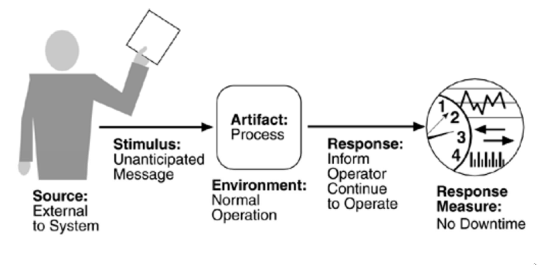
\includegraphics[width=0.6\textwidth]{images/heartbeat-system-concrete-scenario.png}
    \caption{سناریو عینی برای قابلیت دسترسی در مثال بالا}
    \label{fig:heartbeatExampleConcreteScenrario}
\end{figure}

\subsection{سناریو عینی ۲: سیستم مدیریت نوبت‌دهی بیمارستان}

یک بیمارستان تصمیم دارد سیستمی برای مدیریت وقت‌دهی به بیماران طراحی کند. سیستم
باید بتواند درخواست‌های وقت‌دهی را به‌صورت آنلاین و در زمان‌های پرترافیک، مثلاً
در ساعات اولیه صبح، پاسخ دهد.

\begin{multicols}{3}
   \begin{enumerate}
    \item عامل تحریک: کسی که درخواست ثبت وقت دهی را دارد می‌تواند کاربر باشد.
    \item محرک: درخواست ثبت وقتی‌دهی
    \item محیط: در زمان‌های پر ترافیک و ساعت اولیه صبح
    \item فرآورده: سروری که باید درخواست‌ها را دریافت کند و نسبت به آن پاسخی دهد
    (که همان سیستم می‌شود).
    \item پاسخ: پاسخ دادن به درخواست‌های وقت‌دهی
    \item معیار پاسخ: به صورت آنلاین و در کمتر از ۲ ثانیه باشد
   \end{enumerate} 
\end{multicols}

\subsection{سناریو عینی ۳: فروشگاه آنلاین با تخفیف لحظه‌ای}

یک فروشگاه آنلاین قصد دارد کمپینی برای تخفیف لحظه‌ای برگزار کند. کاربران باید
بتوانند در مدت‌زمان محدود (مثلاً 5 دقیقه)، سفارش خود را ثبت کنند و سیستم باید
این سفارش‌ها را به‌سرعت پردازش کند، حتی در زمانی که ترافیک کاربران به‌شدت بالا
می‌رود.

\begin{multicols}{3}
    \begin{enumerate}
        \item عامل تحریک: کاربران
        \item محرک: درخواست ثبت سفارش (ریکوئستی که ارسال می‌شود)
        \item محیط: نرمال و حتی در ترافیک
        \item فرآورده: سرور یا سیستم نرم‌افزاری که خدماتی را ارائه می‌دهد.
        \item پاسخ: پردازش کردن درخواست کاربران نسبت به هر سفارش
        \item معیار پاسخ: به سرعت پردازش کردن سفارش‌ها
    \end{enumerate} 
\end{multicols}

\subsection{سناریو عمومی برای ویژگی کیفی دسترس‌پذیری}

\begin{LTR}
    \begin{table}[H]
        \centering
        \begin{tabular}{|>{\raggedright\arraybackslash}p{0.25\textwidth}|>{\raggedright\arraybackslash}p{0.7\textwidth}|}
            \hline
            \textbf{Portion of Scenario} & \textbf{Possible Values} \\
            \hline
            Source & Internal/external: people, hardware, software, physical infrastructure \\
            \hline
            Stimulus & Fault: omission, crash, incorrect timing, incorrect response \\
            \hline
            Artifact & System’s processors, communication channels, persistent storage, processes \\
            \hline
            Environment & Normal operation, startup, shutdown, repair mode, degraded operation, overloaded operation \\
            \hline
            Response & Prevent the fault from becoming a failure \\
            & \textbf{Detect the fault:} \\
            & \quad $\bullet$ Log the fault \\
            & \quad $\bullet$ Notify appropriate entities (people or systems) \\
            & \textbf{Recover from the fault:} \\
            & \quad $\bullet$ Disable source of events causing the fault \\
            & \quad $\bullet$ Be temporarily unavailable while repair is being effected \\
            & \quad $\bullet$ Fix or mask the fault/failure or contain the damage it causes \\
            & \quad $\bullet$ Operate in a degraded mode while repair is being effected \\
            \hline
            Response Measure & Time or time interval when the system must be available \\
            & Availability percentage e.g., $99.999\%$ \\
            & Time to detect the fault \\
            & Time to repair the fault \\
            & Time or time interval in which system can be in degraded mode \\
            & Proportion e.g., $99\%$ or rate e.g., up to $100$ per second of a certain class of faults that the system prevents, or handles without failing \\
            \hline
        \end{tabular}
        \caption{Scenario Portions and Their Possible Values}
        \label{tab:scenario-possible-values}
    \end{table}
\end{LTR}

\subsection{تاکتیک‌ها}

برای هر ویژگی کیفی مجموعه‌ای از تاکتیک‌ها را می‌توانیم داشته باشیم. هر تاکتیک
روی یک ویژگی کیفی مشخص اعمال می‌شود. اگر چند ویژگی کیفی در سیستم داریم بایستی
\lr{Architectural patterns} را مورد نظر قرار بگیریم.

ویژگی کیفی کارایی را در نظر داشته باشید، برای اینکه بتوانیم به عدد بالایی در
کارایی برسیم باید تاکتیک زمانبندی را انتخاب کنیم که در هر تاکتیک مجموعه‌ای از
استراتژی‌هایی وجود دارد که می‌توان با استفاده از آن‌ها به ویژگی کیفی مورد نظر
رسید. برای مثال در تعیین استراتژی در تکنیک زمانبندی می‌توانیم از الگوریتم
\lr{Shortest Job First (SJF)} استفاده کنیم.

تاکتیک‌ها معمولاً به صورت ترکیبی مورد استفاده قرار می‌گیرند. اینکه ما به چه
صورت از \lr{Monitoring} استفاده می‌کنیم بستگی به سناریو مطرح شده در ویژگی کیفی
مورد نظر دارد.

\subsection{۴ نوع \lr{Fault} نرم‌افزاری}

\subsubsection{\lr{Omission}}

زمانی رخ می‌دهد که یک کامپوننتی نسبت به یک ورودی پاسخ نمی‌دهد.

\subsubsection{\lr{Crash}}

اگر تمام کامپوننت‌ها از \lr{Omission} رنج ببرند سیستم به \lr{Crash} بر می‌خورد.

\subsubsection{\lr{Timing}}

اگر یک کامپوننت بعد از دریافت ورودی، هنگام تولید خروجی زمان غیرمنطقی را سپری کند
با \lr{Fault} مربوط به زمان رو به رو خواهد بود.

\subsubsection{\lr{Response}}

اگر کامپوننت بعد از دریافت ورودی، خروجی که تولید می‌کند پاسخ مناسب و صحیح نباشد
در حقیقت \lr{Response fault} رخ می‌دهد. که خطرناک‌ترین حالت ممکن این \lr{Fault}
نرم‌افزاری است و باید از تکنیک‌هایی استفاده کنیم که این نوع از \lr{Fault} را در
نرم‌افزار خود تشخیص دهیم.

\subsection{مهم‌ترین هدف تاکتیک دسترس‌پذیری}

یکی از مهم‌ترین اهداف دسترس‌پذیری شناسایی تمام \lr{Fault}ها و پوشش آن‌ها
می‌باشد.  حتی زمانی که سیستم به \lr{Fault} بر خورد کرد بتوان خیلی سریع آن را
\lr{Repair} کرد و سیستم را به مدار بازگردانیم.

\subsection{دسته‌بندی تاکتیک‌های دسترس‌پذیری}

تاکتیک‌های ویژگی کیفی «دسترس‌پذیری» ۳ دسته زیر هستند:

\subsubsection{\lr{Detect Faults}}

\begin{enumerate}
    \item \lr{Ping/echo}: یک پیام به عنوان \lr{Async Request/Response} بین
    نود‌ها ارسال می‌شود برای اینکه دریابیم نودی در دسترس است یا خیر. یک پیام
    می‌فرستد تا \lr{ACK} از مقصد دریافت کند و اگر نود مقصد جواب دهد یعنی نود در
    دسترس است. بیشتر برای بدست آوردن \lr{Delay} در شبکه مورد استفاده قرار
    می‌گیرد.
    \item \lr{Monitor}: پایش وضعیت سلامت یک کامپوننت (سیستم، نرم‌افزار،
    سخت‌افزار، شبکه و هر چیزی). اکثراً از این استراتژی برای پیدا کردن حملات
    \lr{DDoS} استفاده می‌شود تا بتوانیم ببینیم منبع حمله از کجا شروع شده است.
    \item \lr{Heartbeat}: برای بررسی صحت ارتباط با نود‌های شبکه مورد استفاده
    قرار می‌گیرد. به صورت دوره‌ای به نود‌های شبکه پیام ارسال می‌کند و دقت
    نمی‌کند که نود‌های مقصد پیام را دریافت کرده‌اند یا خیر.
    \item \lr{Timestamp}: برای متوجه شدن از توالی اشتباه در \lr{Event}ها مورد
    استفاده قرار می‌گیرد. در بحث \lr{Distributed Message Passing} مورد استفاده
    قرار می‌گیرد.
    \item \lr{Sanity check}: بررسی سلامت؛ عملیات یک کامپوننت یا \lr{Output} را
    از نظر منطقی و قابل تایید بودن بررسی می‌کند. ذات و ماهیت اطلاعاتی که دریافت
    کرده‌ایم را با دقت بررسی می‌کنیم. که معمولاً بر اساس دانش طراحی داخلی، وضعیت
    سیستم و یا طبیعت داد‌ها می‌باشد. (مثال ارتفاع اندازه‌گیری شده اشتباه در
    هواپیما با استفاده از این تاکتیک قابل بررسی می‌باشد)
    \item \lr{Condition Monitoring}: چک کردن شرایطی که سیستم مورد نظر در آن قرار
    می‌گیرد که بررسی کنیم آیا مفروضات در طول طراحی حفظ شده‌اند یا خیر. برای مثال
    یخچالی که به تازگی خریداری شده است داغ می‌شود. باید بررسی کنیم که براساس
    مفروضات محصول، آیا فاصله مشخصی را با دیوار دارد یا خیر. زمانی که سیستم‌ها
    ناهمگن هستند مفروضات بایستی رعایت شوند.
    \item \lr{Voting}: این تاکتیک برای بررسی کامپوننت‌هایی مورد استفاده قرار
    می‌گیرد که نتایج یکسانی را تولید می‌کنند. مهم‌ترین نکته این تاکتیک آن است که
    تعداد سیستم‌هایی که در آن در نظر می‌گیریم باید فرد باشند به همین خاطر به آن
    \lr{TMR} یا \lr{Triple Modular Redundency} می‌گویند. دلیل استفاده از ۳ ماژول
    آن است که بیشتر از ۳ ماژول مانند ۵ و ۷ ماژول هزینه بیشتری را تولید می‌کند.
    به عبارتی ساده‌تر زمانی از این سیستم استفاده می‌کنیم که نیاز به سرویس‌های
    بک‌آپ داریم و جوابی که بدست می‌آید درست و غلط آن را نمی‌دانیم. این تاکتیک در
    ۳ روش مختلف می‌تواند بکار گرفته شود:
    \begin{enumerate}
        \item \lr{Replication}: در این حالت هر کامپوننت دقیقاً کلون کامپوننت اول
        می‌باشد. پس ورودی و تابع یکسانی دارند و حتی دقیقاً یک خروجی را تولید
        می‌کنند. اگر در سخت افزار باشد باید جایگزینی نسبت به هم وجود داشته باشد.
        فرمی از تنوع تابع و ورودی و خروجی وجود ندارد. هیچ واگرایی نسبت بهم
        ندارند و از نظر ماهیتی یک چیز هستند.
        \item \lr{Functional redundancy}: در این روش ورودی‌ها یکسان هستند حتی
        خروجی‌ها هم یکسان هستند ولی توابع و الگوریتم‌هایی که در آن‌ها استفاده
        می‌شود متفاوت است. این روش برای زمانی مناسب است که اگر خطایی در یک تابع
        وجود داشته باشد در تابع کامپوننت‌های دیگر نباشد زیرا روش‌های
        محاسبه در کامپوننت‌های دیگر با توابع دیگر متفاوت است اما در انتها همه
        سیستم‌ها یک خروجی را تولید می‌کنند. استفاده از این روش نسبت به
        \lr{Replication} بهتر است زیرا اگر یک تابع کار نکند توابع دیگر ما را به
        خروجی می‌رسانند.
        \item \lr{Analytic redundancy}: در این روش، ورودی، خروجی، و توابع
        پیاده‌سازی شده کاملاً متفاوت هستند و هر سیستمی براساس ورودی مشخص
        (متفاوت) خروجی (متفاوت و متناسب با ورودی) تولید می‌کند. برای مثال در
        هواپیما وقتی فشارسنج و سیستم ارتفاع‌سنج بررسی می‌شود که وضعیت هواپیما را
        ایمن اعلام کنند دقیقاً دو ابزار سیستم استفاده شده حاوی \lr{Workload}
        متفاوت و پردازش متفاوت و خروجی متفاوت با یکای مختلف هستند، اما از این
        سیستم‌ها استفاده می‌شود تا ارتفاع درست هواپیما را اطمینان حاصل کنند. در
        حقیقت این روش در کنار \lr{Sanity checking} بکار می‌رود که بخاطر حیاتی
        بودن مسئله، خلبان از نتیجه‌ای که باید بعد از ۱۵ دقیقه بدست آید، اطمینان
        حاصل کند.
    \end{enumerate}
    \item \lr{Exception detection}: وقتی که یک سیستم از فرایند و عملیات نرمالی
    که انتظار داریم در حال خارج شدن است که می‌توان در برنامه‌نویسی آن را با
    استفاده از \texttt{try-catch} شناسایی نمود و سیستم را در حالت کارکرد درست
    برای کاربر قرار دهیم.
    \item \lr{Self-test}: در حقیقت در این تاکتیک یک مولفه قصد آزمون خودش را دارد
    که از صحت عملکرد خودش تایید را دریافت کند. این تاکتیک در کنار تاکتیک
    \lr{Condition monitoring} می‌تواند مورد استفاده قرار گیرد. این ترکیب در
    سیستم عامل وجود دارد. برای مثال زمانی که رم داخل کامپیوتر نباشد قبل از
    بوت شدن سیستم عامل، در فرایند‌های \lr{BIOS} بررسی می‌شود و صدایی از نوع خطر
    را پخش می‌کند و می‌تواند پیامی را در آن بابت در صفحه نمایش مشاهده کرد. نکته
    مهم آن است که \lr{Self-monitoring} را در کنار آزمون استفاده می‌کنیم تا مطمئن
    شویم عامل خارجی در جهت ایجاد \lr{fault} وجود نداشته باشد.
\end{enumerate}

\subsubsection*{نکات}

\begin{itemize}
    \item در تاکتیک \lr{Voting} بخش \lr{Replication} تنوعی ندارد و در سیستم‌های
    سخت‌افزاری و نرم‌افزاری مورد استفاده قرار می‌گیرد.
    \item یکی از استراتژی‌هایی که در \lr{Availability} وجود دارد تعدیل بار کاری
    در سیستم می‌باشد.
\end{itemize}

\subsubsection{\lr{Recover from Faults}}

\begin{enumerate}
    \item \lr{Preparation and Repair}: آماده‌سازی و تعمیر
    \begin{enumerate}
        \item \lr{Protection group}: در حقیقت در گروهی از گره‌های در شبکه اشاره
        دارد که برخی دائماً \lr{Active} هستند و برخی دیگر به عنوان یدکی یا
        \lr{Spare} استفاده می‌شوند. یکسری از منابع در سیستم فعال هستند و در حال
        انجام تسک‌ها می‌باشند و یکسری از سیستم‌ها در این گروه حکم دستگاه‌های
        پشتیبان یا \lr{Backup} را دارند. اگر گره‌ای که \lr{Active} بوده است از
        کار بیوفتد سریعاً باید دستگاه یدکی به عنوان جایگزین گره قبلی آماده‌سازی
        شود تا سرویس قطع نشود که یکی از شرایط منفی در \lr{Availability} محسوب
        می‌شود. \lr{Fault}های نرم‌افزار دلیل اصلی از کار افتادن گره‌های
        \lr{Active} هستند که در نهایت تبدیل به \lr{Failure} شده‌اند. پس بایستی
        دستگاه‌هایی وجود داشته باشند که بجای دستگاه‌های اصلی وارد مدار شوند تا
        سیستم را ریکاور کنند.
        \begin{enumerate}
            \item \lr{Active redundancy or Hot spare (1+1 redundancy)}: در این
            تکنیک تمام سیستم‌های حاضر در شبکه در حال کار می‌باشند و تمام این
            گره‌ها کلونی از یکدیگر هستند تماماً اطلاعات را بین خودشان \lr{Sync}
            و هماهنگ می‌کنند تا اگر سیستمی از کار افتاد سیستم بعدی‌ای که در مدار
            بوده است و باقی مانده است بتواند ادامه آن کار را بدون وقفه و قطعی
            سرویس انجام دهد. هزینه در این تاکتیک زیاد است اما قدرت
            \lr{Availability} بسیار زیاد است که می‌توان از این نوع تاکتیک‌ها در
            بانک‌ها نیز استفاده کرد چرا که دائماً نیازمند دردسترس بودن هستند. در
            این تاکتیک به ازای هر گره یک گره به عنوان گره \lr{Redundent} وجود
            دارد که وقتی گره \lr{Active} از کار افتاد گره \lr{Spare} که دائماً
            در حال \lr{Sync} شدن بوده است وارد مدار می‌شود.
            \item \lr{Passive redundancy or Warm spare}: در این تاکتیک گره‌های
            موجود در شبکه در حال کار می‌باشند اما تنها در بازه معینی از هفته یا
            یک زمانبندی مشخص داده‌ها را بین خودشان \lr{Sync} و هماهنگ می‌کنند.
            \item \lr{Spare or Cold spare}: در اصل گره‌های یدکی \lr{Out of the
            service} هستند. اصلاً به صورت \lr{Active} یا \lr{Passive} اطلاعات و
            وضعیت آن‌ها \lr{Sync} نمی‌شود، تا زمانی که یک \lr{Fault} در گره
            \lr{Active} رخ دهد و تبدیل به \lr{Failure} شود. به محض این اتفاق،
            گره‌هایی که خاموش بوده‌اند بایستی سریعاً وارد محیط عملیاتی شوند و
            تنها بتوانند عملیات محدود و اولیه و ضروری که در سیستم تعریف شده است
            را به صورت کامل انجام دهد. برای مثال سیستم اسنپ فود اگر به مشکلی
            برخورد کند و از دسترس خارج شود، سریعاً باید سیستم‌های یدکی آماده
            شوند و وارد مدار شوند تا مشتریانی که در هنگام پرداخت پول از حساب
            آن‌ها پرداشت شده اما محصول انتخاب شده از لیست پاک شده‌است سریعاً پول
            به حساب آن‌ها برگردد تا مجدداً در زمان مناسب اقدام به سفارش خود
            کنند. در این لحظه یعنی سرویس \lr{payment} سعی شده است که کامل در
            دسترس اما با قابلیت حیاتی اصلی خودش و محدود در مدار باشد. یعنی
            نمی‌توان در این سناریو از \lr{Cold spare} انتظار داشته باشیم که لیست
            سفارش انتخاب کاربر نیز ریکاور شود.
        \end{enumerate}
        \item \lr{Exception handling}: استراتژی مناسب بعد از تشخیص
        \lr{Exception} در مرحله قبلی را انتخاب می‌کند. برای مثال اگر درخواست از
        کلاینت به سرور با شکست رو به رو شد در قسمت \lr{Exception} پیام مناسبی را
        به کاربر نشان دهد که شاید ممکن است اینترنت کاربر دچار مشکل شده باشد.
        \item \lr{Rollback}: بازگشت به منطقه امن قبلی در نرم‌افزار می‌باشد.
        وضعیت خوب شناخته شده در نرم‌افزار. تمام تراکنش‌ها خاصیت \lr{Rollback} را
        ندارند. برای مثال از حساب بانکی ۵۰ تومان کم شده است و به سیستم دیگری
        هنگام انتقال قطع شده است، باید پول به مبدا برگردد. در حقیقت طراح مشخص
        می‌کند که منطقه و وضعیت امن نرم‌افزار کجا قرار دارد.
        \item \lr{Software upgrade}: وقتی می‌خواهیم \lr{Fault}ی که در سیستم وجود
        دارد را ریکاور کنیم بایستید سیستم را آپگرید کنیم که به وضعیت مطلوب خودش
        برسد.
        \item \lr{Retry}: مهم‌ترین استراتژی تاکتیک \lr{Recovery from Fault}
        می‌باشد. جایی که \lr{Failure} رخ داده‌است را قطع می‌کنیم و دوباره اجرا
        می‌کنیم که به موفقیت برسد. آنقدر \lr{Retry} یا اصطلاحاً تلاش مجدد می‌کند
        تا به موفقیت برسد. برای مثال در سیستم‌آموزشیار، اگر در کلاینت مشکلی
        مشاهده شود، کاربر آنقدر تلاش می‌کند که دوباره بتواند صفحه انتخاب واحد را
        ببیند.
        \item \lr{Ignore faulty behavior}: نسبت به رفتار‌هایی که به نظر
        \lr{Faulty} به نظر می‌رسند آن‌ها را نادیده می‌گیرد. سیستم نسبت به
        پیام‌های مشکوک هیچ واکنشی نشان نمی‌دهد. منبع مشکوک منبعی است که در سیستم
        ناشناخته می‌باشد و احتمالاً سیستم را به سمت \lr{Failure} می‌برد.
        \item \lr{Degradation} یا تنزل: زمانی که یک مولفه در سیستم نرم‌افزاری
        دچار مشکل می‌شود به خاطر آن کل سیستم را \lr{Out of the service} نمی‌کنیم
        بلکه تنها آن قسمت را از دسترسی خارج می‌کنیم که مشکلش را پیدا کنیم و آن
        را حل کنیم. برای مثال زمانی که سینک آشپزخانه یک خانه خراب است کل خانه را
        به خاطر آن نمی‌بندیم که هیچ کس نتواند در آن زندگی کند. اگر به یاد داشته
        باشید نرم‌افزار \lr{Gmail} گوگل یک آیتم در اختیار کاربر قرار می‌داد که
        آن آیتم این امکان را داشت کاربر بتواند با کندترین اینترنت ایمیل‌هایش را
        در محیطی بسیار ساده و ابتدایی دریافت کند. اگر سیستم اصلی گوگل با امکان
        زیاد از کار می‌افتاد این با این آیتم کاربر همیشه در شبکه با امکانات
        محدودتر حاضر بود.
        \item \lr{Reconfiguration}: واگذاری و اختصاص مجدد وظایف به منبع باقی
        مانده. در حقیقت همانند رفتار در \lr{Spare} را دارد، زمانی که یک گره هیچ
        وقت زیر بار نبوده و یک گره \lr{Active} از کار بیوفتد، از گره‌ای که به
        عنوان یدکی در سیستم معرفی شده بود می‌توانیم استفاده کنیم و ادامه کار‌ها
        را در آن ارجاع بدهیم. هر کدام از گره‌ها هنگام واگذاری و اختصاص مجدد
        وظایف ممکن است تنها یکسری کار‌های محدودی را انجام دهند.
    \end{enumerate}
    \item \lr{Re-introduction}: باز معرفی مولفه در سیستم
    \begin{enumerate}
        \item حالت \lr{Shadow}: مولفه‌ای که از دسترسی ما خارج شده است را در یک
        بازه زمانی در حالت \lr{Shadow} قرار می‌دهیم که ورودی‌های جدید از این به
        بعد در این سیستم نیز وارد شوند و بررسی کنیم که آیا آن گره \lr{Active}ی
        که به خروجی مورد نظر رسیده است این گره نیز به آن خروجی می‌رسد یا خیر؟
        کاربرد بسیار زیادی برای سیستم‌هایی که در دامنه‌های بحرانی و
        \lr{Critical} استفاده می‌شوند دارد با اینکه هزینه زیادی بابت روشن بودن
        چندین گره دارد اما \lr{Availability} بالایی را نیز همراه خواهد داشت.
        \item \lr{State resync}: این تاکتیک زمانی استفاده می‌شود که سیستم‌هایمان
        در \lr{Protection group} در حالت‌های \lr{Active} و \lr{Passive
        redundent} هستند. این تاکتیک می‌تواند به \lr{Monitoring} وابسته باشد که
        در ابتدا اطلاعات را بررسی کند و سپس بعد از آن عمل \lr{Resync} را انجام
        دهد.
        \item \lr{Non Stop Forwarding (NSF)}: اگر بخواهیم یک سیستمی را بررسی
        کنیم که الگوریتم آن به واسطه ورودی‌هایی که روی آن انجام می‌شوند، فعال
        می‌شود از این تاکتیک استفاده می‌کنیم. برای مثال زمانی که یک مسیریاب
        الگوریتمش به درستش کار نکند و به هر دلیلی الگوریتم مسیریابی آن با شکست
        مواجه شود سیستم باید سعی کند با جدول همسایگی که از گره‌ها دارد از یک
        الگوریتم جایگزین استفاده کند که بسته را از مبدا به مقصد برساند. نکته مهم
        در \lr{NSF} آن است که سعی شود هیچ وقت ارتباطات از بین نرود و گره اگر هر
        اتفاقی برایش افتاد مسیر جدیدی را پیدا کند.
        \item \lr{Escalating restart}: به معنای بالا آوردن سیستم یا اضافه کردن
        می‌باشد. عموماً در سیستم با سلسله مراتب مواجه می‌شویم که والد فرزندی
        هستند. طراح تصمیم می‌گیرد که وقتی یک سیستم تنزل آبرومندانه کرده باشد
        باید سلسله مراتبی \lr{Up \& Running} شود که مولفه به مولفه صورت می‌گیرد.
        یعنی اول بچه‌ها و بعد والد و به ترتیب به بالاترین عضو درخت یا \lr{root}.
        این اصطلاح را معمولاً به \lr{Graceful degradation} می‌شناسند.
    \end{enumerate}
\end{enumerate}

\subsubsection*{نکات}

\begin{itemize}
    \item هزینه‌ها در \lr{Protection group} به ترتیب گفته شده از زیاد به کم است.
    \item عموماً در سیستم یک تاکتیک استفاده نمی‌شود بلکه مجموعه‌ای از تاکتیک‌ها
    می‌توانند در کنار هم دیگر قرار گیرند تا از بروز \lr{Fault} و تبدیل شدنش به
    \lr{Failure} جلوگیری کنند. سیستم هر موقع به آن آستانه رسید باید استراتژی
    مناسبی را آماده داشته باشیم که سیسیتم را از آن شلوغی و اختلالی که رخ داده
    است آزاد کنیم. آستانه‌ها کاملاً وابسته به مشاهدات و تجربه مهندس است.
    \item کاملاً به سیستم وابسته است، هیچ وقت \lr{Single criteria} عمل نمی‌کنیم.
\end{itemize}

\subsubsection{\lr{Prevent Faults}}

\begin{enumerate}
    \item \lr{Removal from service}: این بخش با جوان‌سازی نرم‌افزار یا
    \lr{Software rejuvenation} ارتباط دارد. برای مثال وقتی یک مولفه‌ای دچار
    \lr{Memory leak} می‌شود سریعاً عامل نشتی آن شناسایی شود سپس هر مشکلی که دارد
    را حل کنیم تا نرم‌افزار به حالت سالم و برنای خودش برسد.
    \item \lr{Transactions}: مباحثی در مورد مسابقه بر سر رسیدن به منابع وجود
    دارد که بتوان به صورت بهینه دو یا چند تراکنش همزمان روی یک منبع عملیات مختلف
    خواندن و نوشتن را انجام دهند. پس بایستی از استراتژی‌های مناسب همروندی و
    مباحث مهم مدیریت توزیع شده تراکنش‌ها مانند \lr{2PC} و \lr{3PC} در موقعتی
    مناسب استفاده شود.
    \item \lr{Predictive model}: مدل‌های پیش‌بینی در هر سیستم کاملاً براساس
    داده‌ها امکان پذیر می‌باشد. این داده‌ها از طریق \lr{Monitoring} مولفه‌ها در
    هر بخشی حاصل می‌شود. اگر ما داده‌های پایش سیستم را بررسی کنیم می‌توانیم
    تصمیم مناسبی را برای مقابله از وقوع هر \lr{Fault} داشته باشیم. برای مثال نرخ
    ورودی داده‌های درخواستی زیاد می‌شود که می‌توانیم از \lr{Monitoring} +
    \lr{Prediction} استفاده کنیم که از حمله‌های \lr{DDoS} جلوگیری به عمل آوریم.
    \item \lr{Exception prevention}: پرهیز از هر گونه \lr{Exception} در کل حاصل
    می‌شود. وقتی ما از \lr{Smart pointer}ها در زبان برنامه نویسی خود استفاده
    کنیم یا از رپر‌ها برای کاهش پیچیدگی کد و \lr{Abstract Data Type (ADT)}ها جهت
    معرفی عملکرد هر کلاس به صورت چکیده استفاده کنیم می‌توانیم سطح پیچیدگی سیستم
    را به شدت کاهش دهیم و از بروز هر گونه \lr{Exception}های ناگهانی در کد
    جلوگیری کنیم.
    \item \lr{Increase competence set}: افزایش مجموعه شایستگی‌ها، در این حالت
    مولفه‌ها را طوری طراحی می‌کنیم که مجموعه شایستگی آن‌ها از حوزه رفتاریشان
    بیشتر شده باشد. فرض می‌کنیم که یک مولفه داریم و می‌خواهیم به آن دسترسی پیدا
    کنیم. در خواست را به مولفه‌ ارسال می‌کنیم که به هر دلیلی \lr{Accept}
    نمی‌شود. برای مثال درخواست قابل انجام نبوده است و دسترسی لغو شده است. مقداری
    صبر می‌کند و مجددا تلاش می‌کند که این درخواست را داشته باشد. در این حالت نرخ
    عدم دسترس‌پذیری مولفه کمتر می‌شود که در فرصتی مناسب دوباره تلاش کرده تا به
    مدار برگشته است. به عبارتی مولفه‌ای داشته باشیم که برای ۲ ثانیه دیگر با تلاش
    مجدد بتواند دسترسی پیدا کند. یعنی طراحی یک مولفه‌ای که بتواند کیس‌هایی مانند
    \lr{Fault}ها را مانند بخش عادی و نرمال سیستم هندل کند.
\end{enumerate}